\documentclass[11pt, oneside]{article} 
\usepackage{geometry}
\geometry{letterpaper} 
\usepackage{graphicx}
	
\usepackage{amssymb}
\usepackage{amsmath}
\usepackage{parskip}
\usepackage{color}
\usepackage{hyperref}

\graphicspath{{/Users/telliott_admin/Dropbox/Tex/png/}}
% \begin{center} 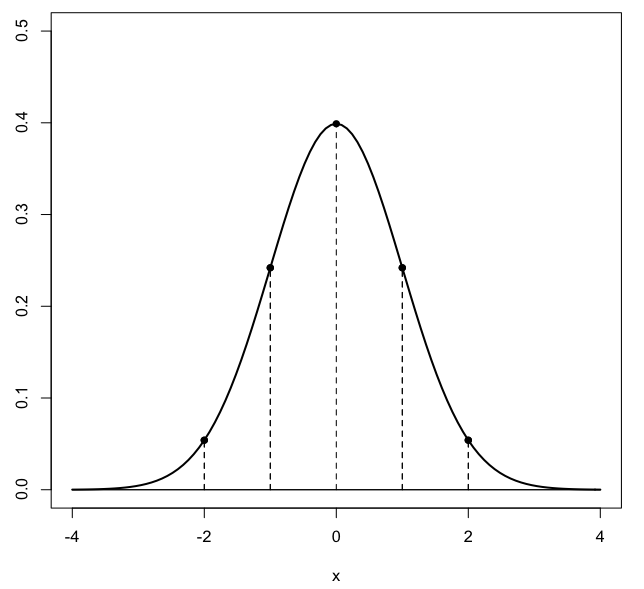
\includegraphics [scale=0.4] {gauss3.png} \end{center}

\title{deMoivre's formula}
\date{}

\begin{document}
\maketitle
\Large

The formula says that for integer $n$
\[ [ \ \cos x + i \sin x \ ]^n = \cos nx + i \sin nx \] 

If we know Euler's formula the derivation is trivial:
\[ e^{i \theta} = \cos \theta + i \sin \theta \]
\[ (e^{i \theta})^n = \ [ \ \cos x + i \sin x \ ]^n \]
\[ = e^{i \theta n}  = e^{in \theta} = \cos n \theta + i \sin n \theta \]

\subsection*{induction}

We can also prove it by induction.  Multiply the first formula above by $(\cos x + i \sin x)$.  The left-hand side is the form we seek.  The right-hand side is
\[ (\cos nx + i \sin nx) \cdot (\cos x + i \sin x) \]
\[ = \cos nx \cos x - \sin nx \sin x + i (\sin nx \cos x + \cos x \sin nx) \]

Using the sum of angles formulas we obtain
\[ = \cos (nx + x) + i \sin (nx + x) \]
\[ = \cos (n+1) x + i \sin (n+1) x \]
which completes the inductive step.

The base can be chosen as $n = 1$.

\subsection*{example}
Let $n = 3$.  Then

\[ [ \ \cos x + i \sin x \ ]^3 = \cos 3x + i \sin 3x \] 
\[ = (\cos^2 x - \sin^2 x + 2i(\sin x \cos x)) \cdot (\cos x + i \sin x) \]

Taking the real part of the last expression we have
\[ \cos 3x = \cos^3 x - \sin^2 x \cos x - 2 \sin^2 x \cos x \]
\[ = \cos^3 x - 3 \sin^2 x \cos x \]

This can be massaged
\[ \cos 3x = \cos x (\cos^2 x - 3 \sin^2 x) \]
\[ = \cos x (\cos^2 x - 3 (1 - \cos^2 x)) \]
\[ = 4 \cos^3 x - 3 \cos x \]

\subsection*{standard formula}
This agrees with the standard formula:
\[ \cos 3x =\cos 2x + x \]
\[ = \cos 2x \cos x - \sin 2x \sin x \]
\[ = (\cos^2 x - \sin^2 x) \cos x - 2 \cos x \sin x \sin x \]
\[ = \cos^3 x - \cos x \sin^2 x - 2 \cos x \sin^2 x \]
\[ = \cos^3 x - 3 \cos x \sin^2 x \]

From here

\url{https://math.stackexchange.com/questions/852122/picture-intuitive-proof-of-cos3-theta-4-cos3-theta-3-cos-theta}

we get a nice geometric derivation.
\begin{center} 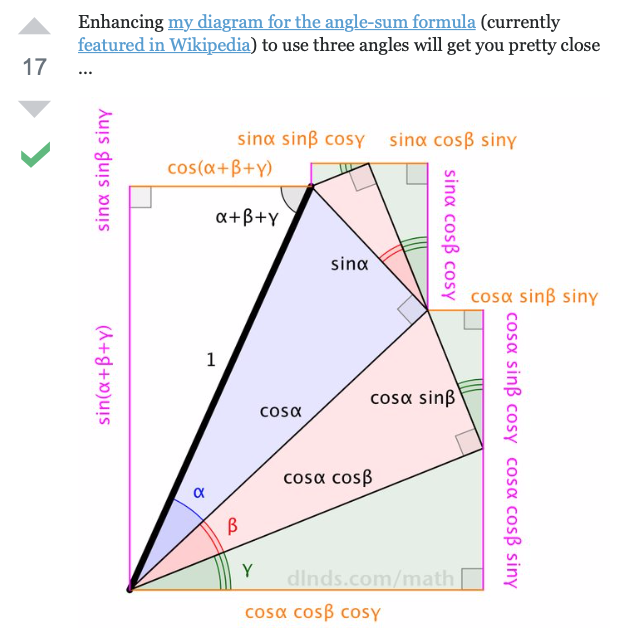
\includegraphics [scale=0.5] {cos3x.png} \end{center}

Note:  the formula is not valid for non-integer powers.

\url{https://en.wikipedia.org/wiki/De_Moivre%27s_formula#Roots_of_complex_numbers}

\end{document}